\section{CritiqueKit: Interactively Guiding Feedback}
Based on these methods and insights, CritiqueKit (Figure \ref{fig:critiquekit_interface}) categorizes feedback and provides prompts and suggestions to reviewers. It differs from prior work by providing feedback to reviewers as they type rather than after they submit. We hypothesize that this contextual assistance may provide a just-in-time scaffold that changes how reviewers' thoughts crystallize, yielding feedback that is more specific, actionable, and/or justified. 

Much like the previous systems in this dissertation, CritiqueKit's interface embeds assistance in the context of the user's task, by displaying interactive guidance and suggestions in a panel next to the work being reviewed. Like DiscoverySpace, CritiqueKit prioritizes ease of use for achieving outcomes; users can reuse a feedback suggestion by simply clicking on it. However, unlike DiscoverySpace, CritiqueKit also helps users improve the feedback they come up with from scratch. As our deployments will show, reviewers are often reluctant to directly reuse feedback suggestions, preferring instead to write their own ideas. While DiscoverySpace does not provide support for users who choose to use Photoshop's tools directly, CritiqueKit explores how simple guidance might help reviewers go beyond direct reuse while still achieving outcomes quickly and easily.

\begin{figure}[b!]
\centering
  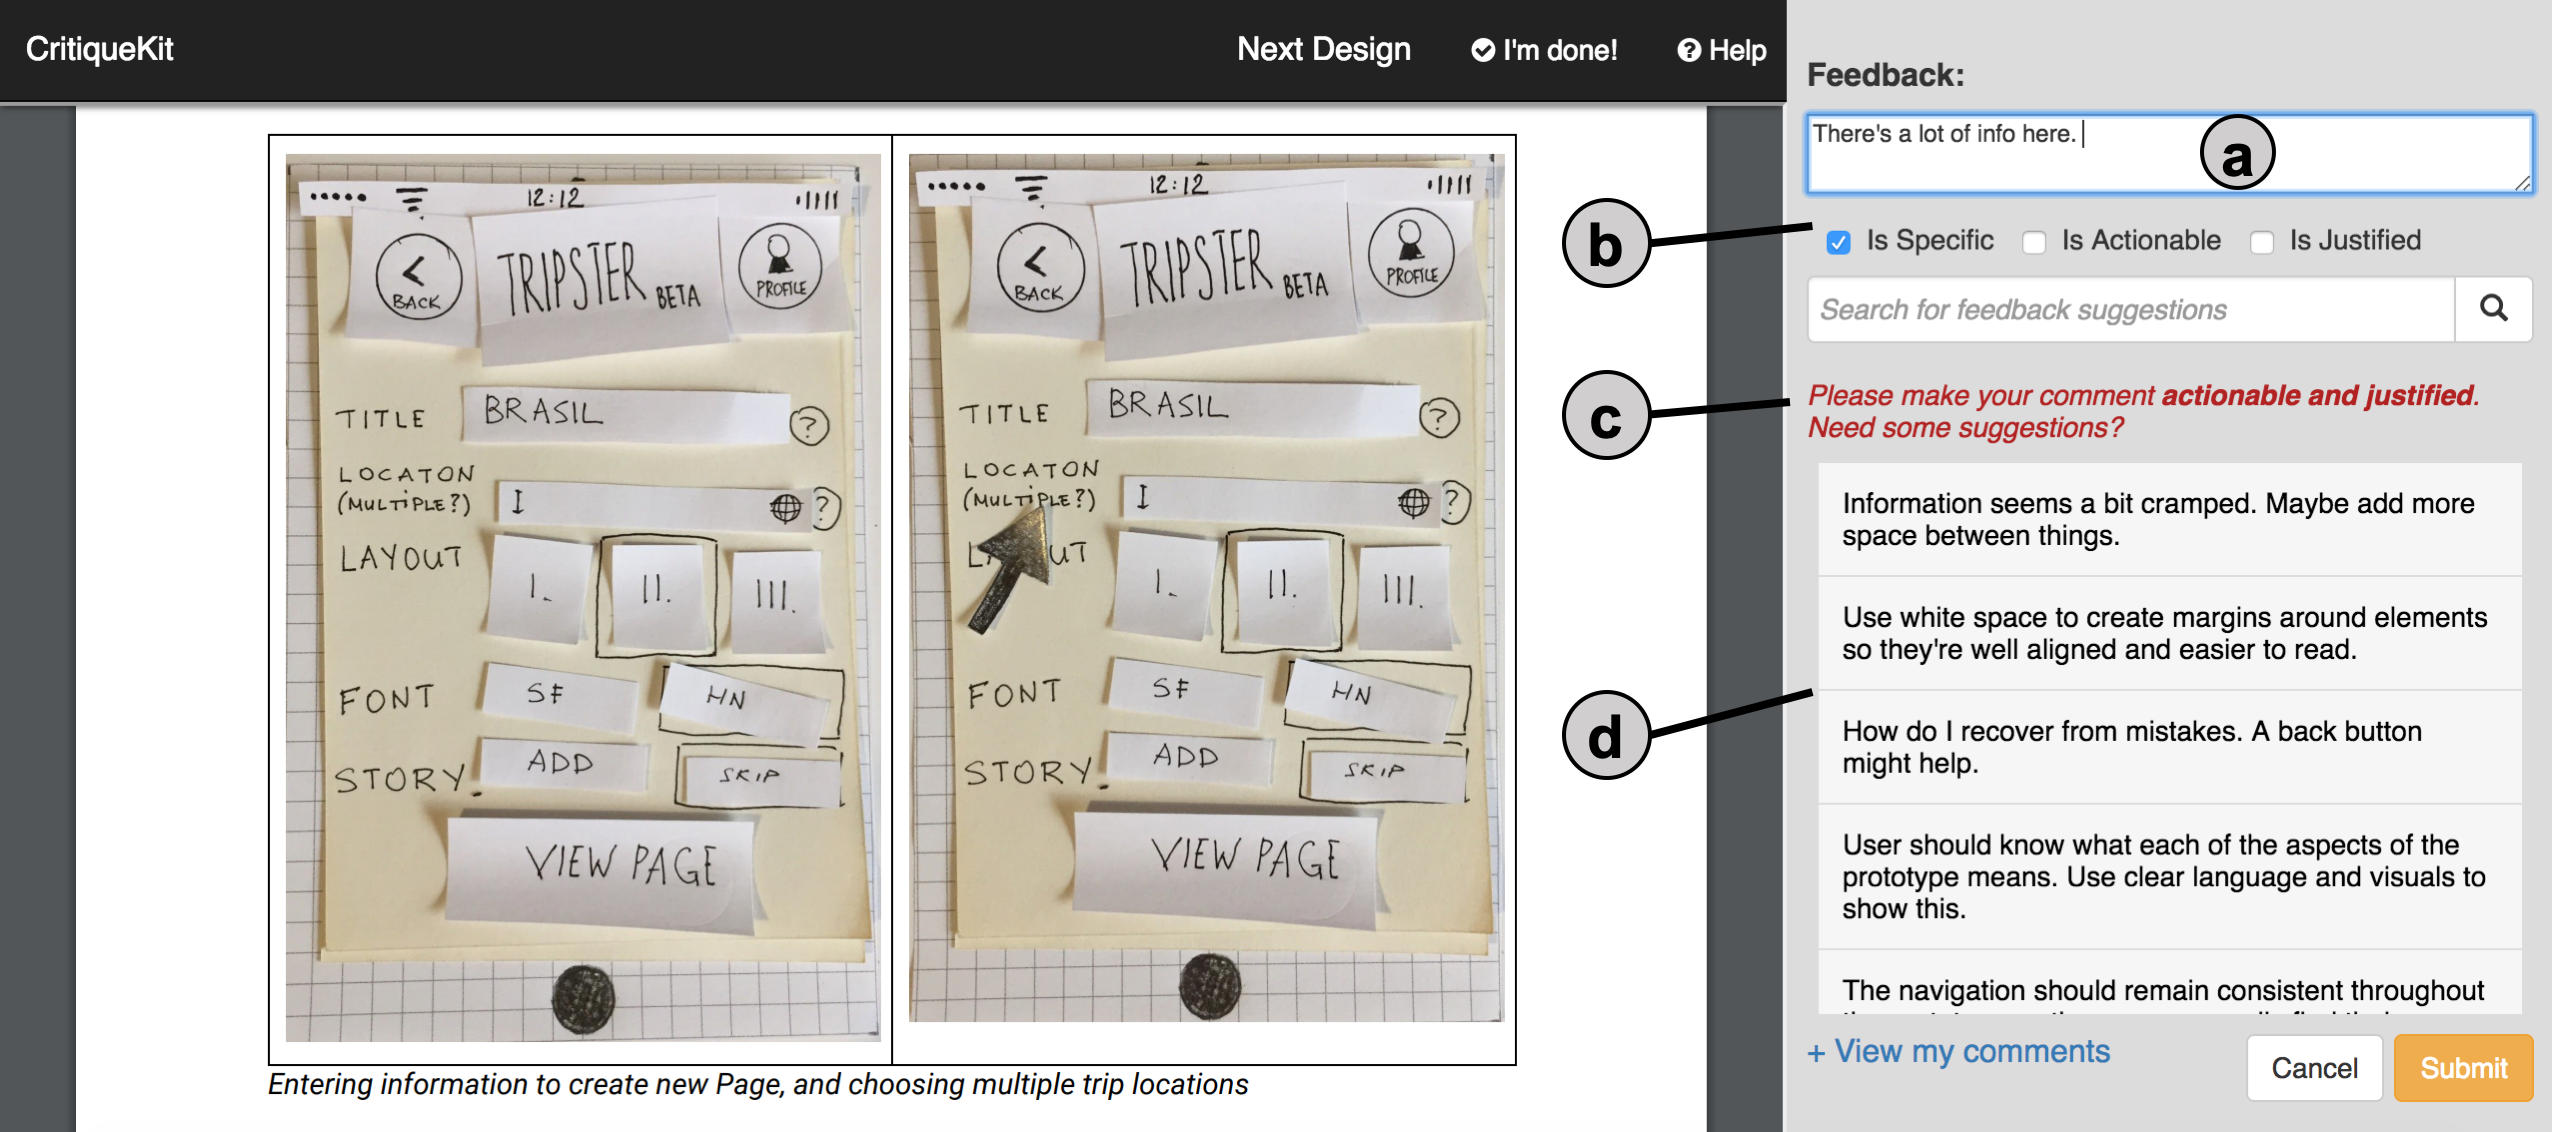
\includegraphics[width=\textwidth]{critiquekit/figures/interface.png}
  \caption[The final CritiqueKit interface (used for Experiment 2).]{The final CritiqueKit interface (used for Experiment 2). a) The reviewer can type their feedback in the textbox. b) The checkboxes in the guidance panel update based on the characteristics of the reviewer’s comments. c) CritiqueKit explicitly prompts reviewers to ensure their comment fits the checkboxes in the guidance panel. d) The reusable feedback suggestions in the suggestions box update based on the unchecked characteristics in the guidance panel, adapting specifically to the reviewer's feedback.}~\label{fig:critiquekit_interface}
\end{figure}

\subsection{Interactive Guidance as a Form of Scaffolding}
CritiqueKit features an interactive guidance panel (Figure \ref{fig:critiquekit_interface}b) with checkboxes that update based on which of three attribute categories the feedback fits: \textit{Is Specific} \cite{Krause2017, sadler1989formative, sommers1980revision, yuan2016}, \textit{Is Actionable} \cite{Dow2012, Gibbs, Kulkarni2015, Luther2015, sadler1989formative, Tseng2007}, and \textit{Is Justified} \cite{Gielen2010, Krause2017, Narciss2006, yuan2016}. 

The prototype assesses the feedback's fit with the following heuristics. The heuristic for the \textit{specific} category merely requires that comments be at least five words long because vague comments tend to be short, such as ``good job'' or ``needs work.'' Perhaps surprisingly, we observed that the five-word nudge was sufficient to garner specific feedback in practice. (Some websites, like Etsy, also use a five-word minimum heuristic for reviews). For the \textit{actionable} and \textit{justified} categories, we manually combed feedback that had been hand-labeled as meeting these categories and observed that specific keywords (i.e., ``maybe try'' and ``you should'' for actionable; ``because'' and ``so that'' for justified) were strong cues of these categories. Consequently, the prototype implementation simply checks for the presence of these keywords and phrases in feedback comments. 

A comment is considered complete once all checkboxes are checked. Reviewers can manually check and uncheck the checkboxes if they feel the checkboxes did or did not add a category in error. For example, if a reviewer's comment states, ``Use a 2-column grid layout,'' and the ``Is Actionable'' checkbox remains unchecked, the reviewer can manually check the checkbox to note that their comment does indeed contain an actionable suggestion. 

\subsection{Adaptive Suggestions for Greater Specificity}
The suggestions box (Figure \ref{fig:critiquekit_interface}d) contains a list of previously given feedback from experts. These suggestions dynamically adapt based on how the reviewer's feedback is categorized in the guidance panel. For example, if a reviewer's comment does not yet satisfy the actionable and justified categories (as in Figure \ref{fig:critiquekit_interface}), the suggestions box would contain examples of feedback with these characteristics. Suggestions appear in the order they were added to the corpus.

\subsection{The CritiqueKit Review Workflow}
When a reviewer first opens CritiqueKit, a prompt asks them to provide specific feedback on something they like about the design and something that could be improved. The suggestions box contains general feedback snippets \cite{kulkarni2013peer} pertinent to the review criteria to give reviewers a starting point, providing suggestions that are broadly applicable and fit within the specified criteria. The ``Submit'' button at the bottom of the interface is red to indicate that the comment text box is either empty or does not fit any of the categories in the guidance panel. 

Once a comment is sufficiently long, the ``Is Specific'' checkbox will check, and the reviewer will be prompted to make their comment actionable and justified. The ``Submit'' button turns yellow to indicate that their feedback is not yet complete, though they can still submit if desired. The feedback suggestions then change to present comments that instantiate both actionable and justified feedback. The suggestions continue to adapt depending on the characteristics of the comment, showing reusable examples of feedback that satisfy the unchecked categories in the guidance panel. The reviewer can insert a suggestion directly into their own feedback by clicking on it. They can then edit the suggestion if they wish in the text field. Once all checkboxes are checked, the ``Submit'' button turns green as an indication of completeness. 

Using prior feedback as suggestions can give inspiration and highlight common issues. The presence of the structured guidance panel reminds reviewers of attributes that feedback should have. 

\subsection{Implementation}
CritiqueKit is a client-server web application implemented using Node.js; it assumes that all content to be reviewed is available on the web. The corpus of reusable feedback comments is stored on the server in \textsc{json} format.

CritiqueKit uses web sockets for communication between each client running the application and the main server, implemented using the socket.io module. Feedback classification happens on the client-side using JavaScript. Feedback suggestions are also generated on the client-side after retrieving the corpus from the server; the suggestions box adaptively shows and hides comments using JavaScript. 

Users access CritiqueKit by navigating to its \textsc{url} in a web browser. The first time the browser loads the website, a unique \textsc{id} is generated for the user and sent to the server. A cookie is also saved on the client-side so that the server can identify and differentiate users. The review content is loaded within the page as an iframe.
